Our mathematical model sheds light on the intricate dynamics of antibiotic resistance and provides a theoretical framework for devising effective intervention strategies. By identifying stable equilibria and delineating distinct biological scenarios, our model offers valuable insights into the interplay between antibiotic-resistant bacteria, the immune response, and antibiotic treatment. Our model is characterized by a system of four differential equations.

\begin{table}[ht]
	\centering
	\caption{The selection of parameters}
	\label{tab:parameters}
	\begin{tabular}{cccc}
		\hline
		\textbf{$E_1$} & \textbf{$E_+$} & \textbf{$E_-$} & \textbf{$E_*$} \\ 
		\hline
		$\alpha = 1$ 	& $\alpha = 0.2$ 	& $\alpha = 1$ 	& $\alpha = 0.1$ \\
		$\beta = 0.1$ 	& $\beta = 0.3$ 		& $\beta = 0.1$ & $\beta = 1.7$ \\
		$\gamma = 1$ 	& $\gamma = 1$ 		& $\gamma = 1$ 	& $\gamma = 1$ \\
		$\eta_s = 1$ 	& $\eta_s = 2$ 		& $\eta_s = 4$ 	& $\eta_s = 3$ \\
		$\eta_r = 0.3$ 	& $\eta_r = 2.5$ 	& $\eta_r = 1$ 	& $\eta_r = 0.5$ \\
		$\mu = 3$ 		& $\mu = 3$ 		& $\mu = 3$ 	& $\mu = 3$ \\
		\hline
	\end{tabular}
\end{table}
0.1, 1.4, 1, 3, 0.5, 3

Initially, we establish the presence of a positively invariant set, indicating a natural constraint on growth due to limited resources, as expressed in the logistic growth term.

\begin{figure}
	\centering
	\caption{Equilibria of $E_1$}
	\label{fig:e1}
	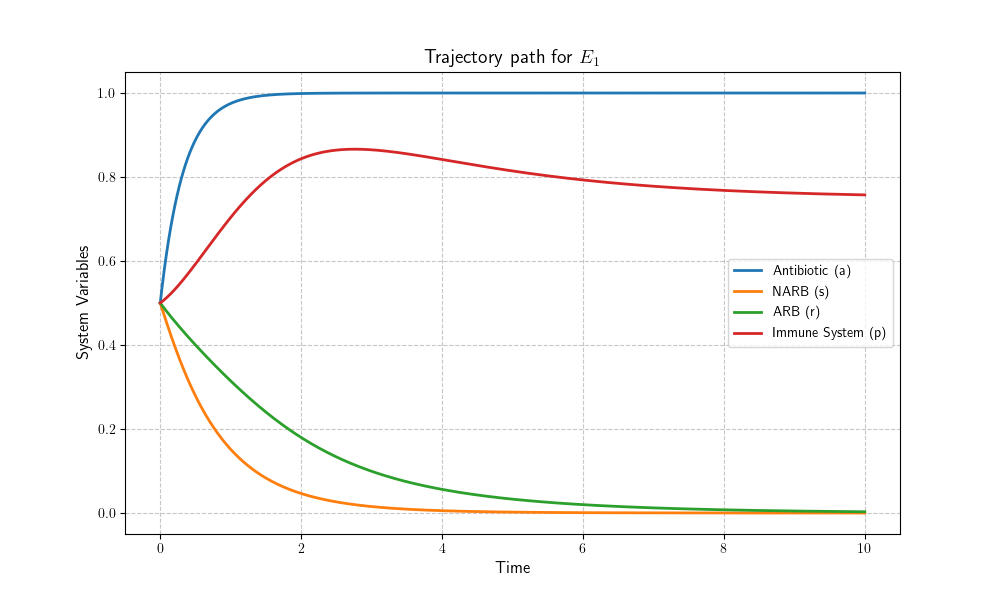
\includegraphics[width = 0.7\textwidth]{E_1.png}
\end{figure}


Additionally, the qualitative investigation reveals the presence of four stable equilibria. The stability of the equilibrium point $E_1 \left(1, 0, 0, f(0)\right)$ is clarified through specific limit calculations, which provide insights into the behavior of the system under certain conditions. This equilibrium represents a state where the infection has been cleared from the system. From a biological perspective, the stability of $E_1$ implies that the system can reach this infection-free state when key parameters align favorably. Specifically, for $E_1$ to be stable, two crucial conditions must be met: First, the antibiotic must be administered at a sufficiently high rate compared to the reproduction rate of non-resistant bacteria. This ensures that the population of non-resistant bacteria is suppressed effectively. Second, the immune response must be strong enough to outcompete and eliminate resistant bacteria. When both of these conditions are satisfied, the system can overcome the infection, leading to the eventual disappearance of the bacterial population.


\begin{figure}
    \centering
    \caption{Equilibria of $E_+$ and $E_-$}
    \begin{subfigure}{0.49\textwidth}\label{fig:epos}
        \centering
        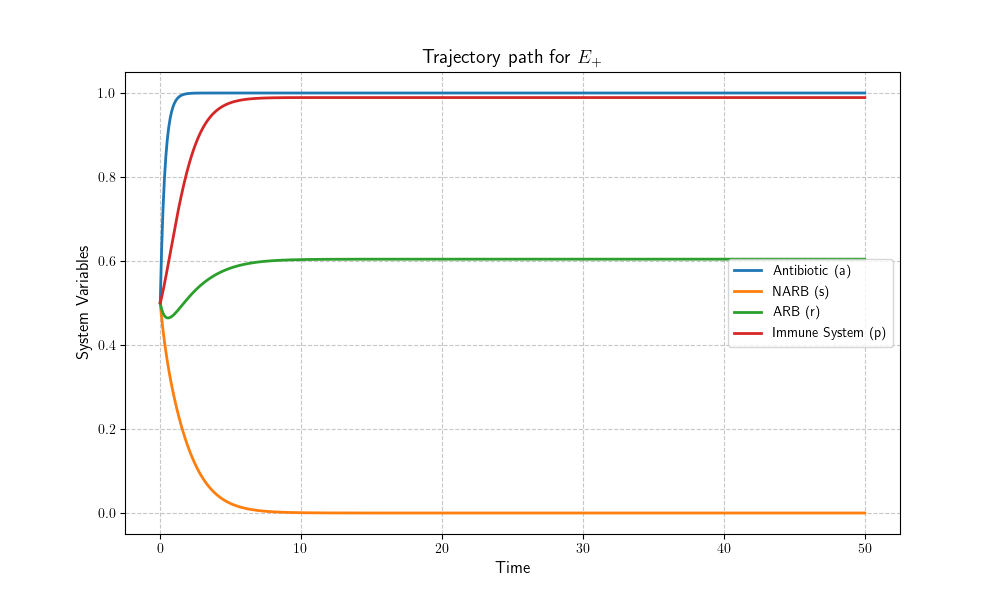
\includegraphics[width =\textwidth]{E_pos.png}
    \end{subfigure}
    \begin{subfigure}{0.49\textwidth}\label{fig:eneg}
        \centering
        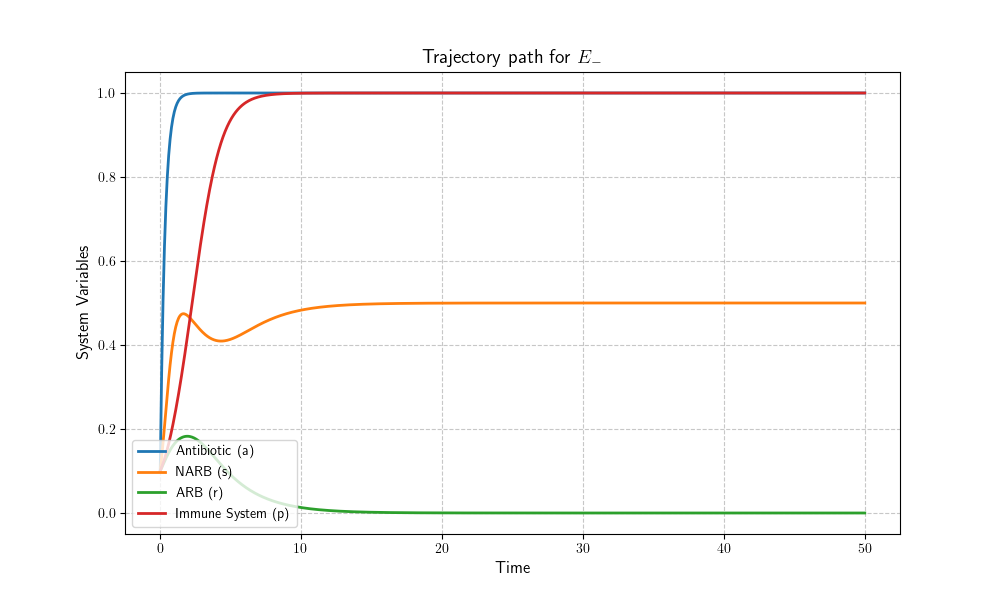
\includegraphics[width = \textwidth]{E_neg.png}
    \end{subfigure}
\end{figure}

The stability analysis of the equilibria $E_+$ and $E_-$ is provided through the Lyapunov theory, which provides a rigorous mathematical framework for assessing the stability of these points in the system. In terms of biology, $E_+$ describes a situation where the infection is sustained entirely by resistant bacteria. At this point, the antibiotic is effective in eliminating non-resistant bacteria, which means that the non-resistant strain is unable to survive in the presence of the treatment. However, the resistant bacteria continue to propagate, suggesting that the antibiotic is not effective against them. This scenario highlights the challenge posed by antibiotic resistance: even with a strong treatment, the infection persists due to the presence of bacteria that can withstand the antibiotic. The stability of $E_+$ implies that under certain conditions—specifically, when the resistant bacteria have a survival advantage—the system will remain in this state unless external interventions are made to counteract the resistance.


In contrast, the equilibrium $E_-$ represents a different biological outcome. Here, the infection is driven entirely by non-resistant bacteria, with the resistant strain being eliminated. This situation arises when the antibiotic dosage is insufficient to suppress the non-resistant bacteria fully, allowing them to continue propagating. However, the resistant bacteria are outcompeted by the immune system because their reproduction rate is lower compared to the strength of the immune response. In this scenario, while the non- resistant bacteria remain problematic, the resistant bacteria do not pose a threat, indicating that the infection can still be controlled if the immune response is sufficiently strong. The stability of $E_*$ suggests that under certain conditions, the system can settle into a state where non-resistant bacteria dominate, but the resistant bacteria are eradicated.

\begin{figure}\label{fig:estar}
    \centering
    \caption{Equilibria of $E_*$}
    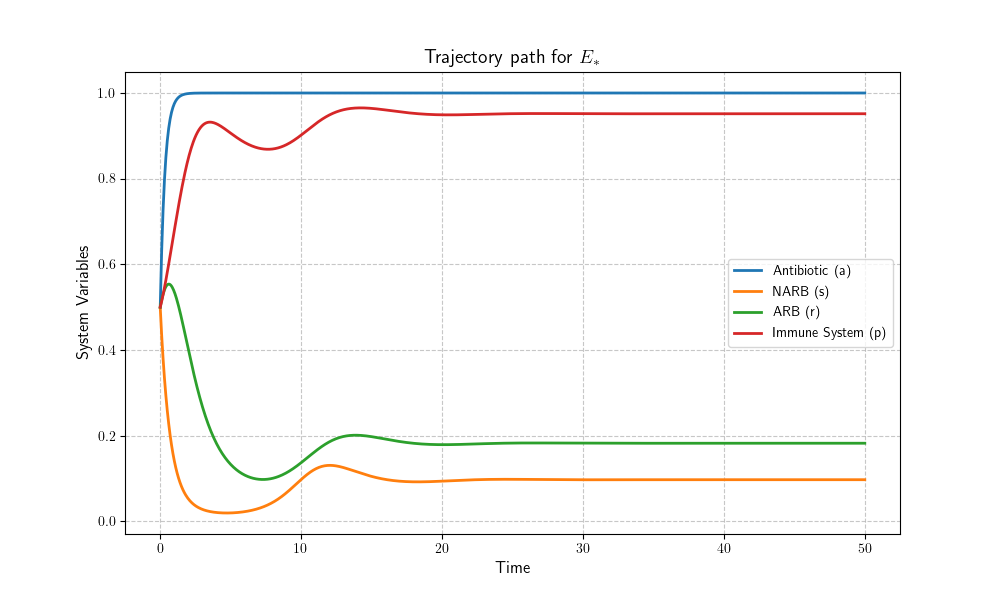
\includegraphics[width = 0.7\textwidth]{E_star.png}
\end{figure}


Ultimately, the stability of $E_* \left(1, s_* , r_* , f (n_*)\right)$ is established through the combined application of the Lyapunov theory and the Routh criteria theorem. In biological terms, the stability of $E_*$ indicates that neither the antibiotic nor the immune response alone can eradicate the infection instigated by both non-resistant and resistant bacteria. In this scenario, a good approach involves incrementally raising the antibiotic dosage within reasonable limits. Indeed, according to the World Health Organization (WHO), widespread antibiotic usage fosters the evolution of resistance in bacteria, prompting them to develop mechanisms to counteract the antibiotic's effects. So ideally, combining the antibiotic with an antivirulence treatment would be optimal. In fact, the latest studies show that employing anti-virulence therapeutic strategies against bacterial infections emerges as the most effective biological approach for eradicating the bacterial infection. Microorganisms possess diverse resistance mechanisms against various classes of antibiotics, underscoring the imperative to uncover novel antimicrobial compounds for combating bacterial infections. A compelling and innovative approach to neutralizing pathogens involves antivirulence therapy, which entails inhibiting bacterial virulence factors or pathogenicity. Consequently, integrating these novel pathoblockers into treatment regimens could diminish the necessity for broad-spectrum antimicrobial administration and curb the prevalence of resistant strains. Introducing antivirulence treatment into our future study would be highly intriguing from a modeling perspective.


Another aspect to consider concerning the equilibrium point $E_*$ is whether the density of resistant bacteria surpasses that of non-resistant bacteria. This holds significant biological importance in combating the infection. In fact, if the condition
\[
2\gamma f\left(1 - \frac{\alpha + \beta}{\eta_S - \eta_T}\right) + \alpha \geq (\eta_S + \eta_T)\frac{\alpha + \beta}{\eta_S - \eta_T} 
\]

is satisfied, then $s_* \ge r_*$.

In future research, exploring the spatiotemporal dynamics of bacterial infection spreading in tissues would be particularly intriguing. Notably, research has demonstrated variations in infection spread across different tissues, organs, and the bloodstream.
